%\documentclass[draft]{beamer}%\documentclass[]{beamer}
\documentclass[]{beamer}%\documentclass[draft]{beamer}
\usepackage{wrapfig}
\usepackage[export]{adjustbox}
\mode<presentation>
{
%  \usetheme{Boadilla}
  \usetheme{Frankfurt}
  \usecolortheme{crane}
}

\setbeamerfont{fig_font}{size=\small}
\setbeamercovered{invisible}
\usefonttheme[onlysmall]{structurebold}
% Delete this, if you do not want the table of contents to pop up at
% the beginning of each subsection:
% \AtBeginSubsection[]
% {
%   \begin{frame}<beamer>{Outline}
%     \tableofcontents[currentsection,currentsubsection]
%   \end{frame}
% }

% End Beamer stuff
\begin{document}
\title{ Physics Behind the Simulation: }
\subtitle{ A CS251 Report by Group 26 }

\author{
	Animesh Baranawal - 130050013 \\
	\texttt {animeshbaranawal@gmail.com} \\
	Rawal Khirodkar - 1300050014 \\
	\texttt {rawalkhirodkar@gmail.com} \\
	Lokit Kumar Paras - 130050047 \\
	\texttt {lokit95@gmail.com} 
}

\date{ 29th September, 2014 }

\begin{frame}
  \titlepage
\end{frame}

\begin{frame}

\frametitle{Overview}
\begin{minipage}{0.5\textwidth}
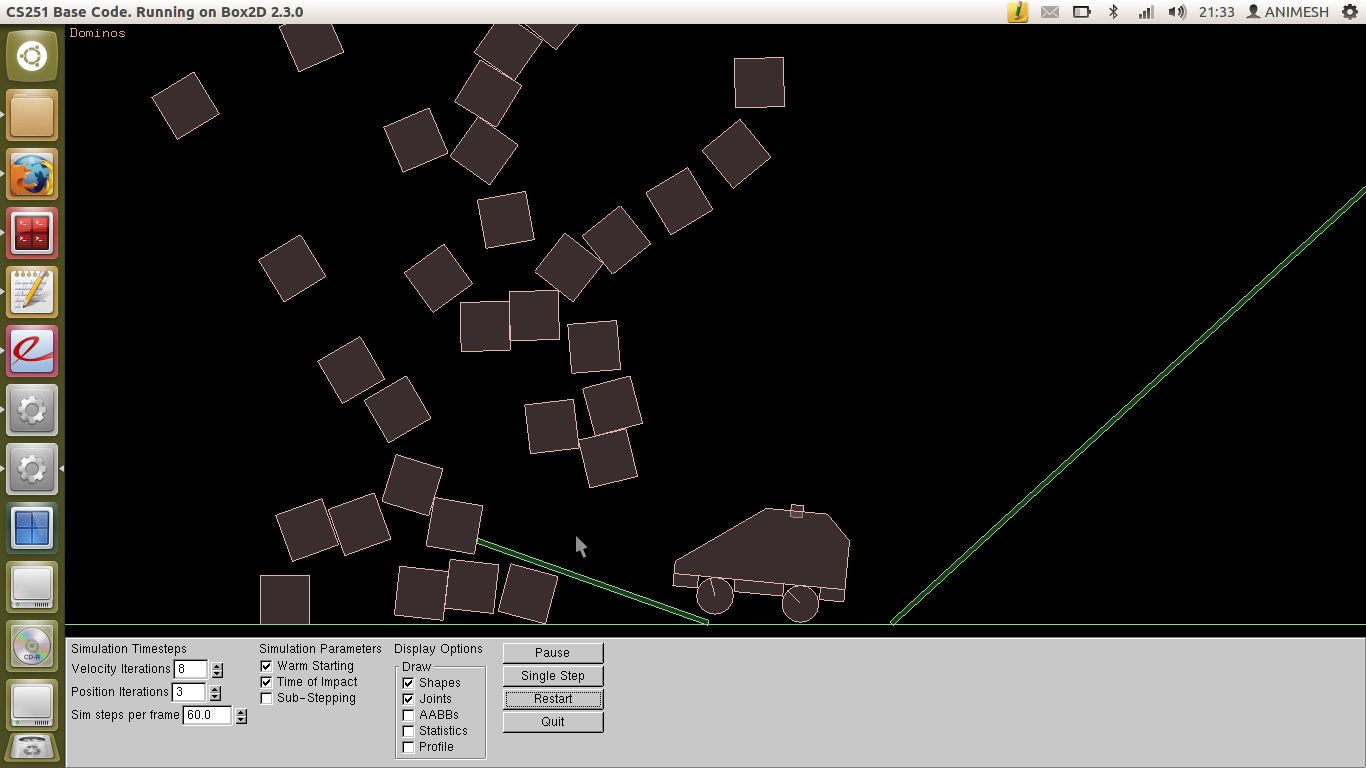
\includegraphics[height=1.0\textwidth,width=1.0\textwidth,right]{./Screenshots/title.png} \pause
\end{minipage}
\begin{minipage}{0.4\textwidth}
\begin{itemize}
  \item Introduction\pause
  \item Divisions \pause
    \begin{itemize}
      \item Limelight Items \pause
        \begin{itemize}
        \item Bike 
        \item Car 
        \item Tank \pause
	\end{itemize}  
      \item Terrain Designing \pause
    \end{itemize}
  \item The Final Picture 
\end{itemize}
\end{minipage}
\end{frame}

\begin{frame}
\frametitle{Introduction}
MOTIVATION BEHIND OUR PROJECT
\begin{itemize}
  \item Appreciating the coolness of a Physics Engine like \textbf{Box2D}. \pause
  \item Implementation of {\em Rube Goldberg Machine} using Box2D with a twist. \pause
  \item \alert{Twist}: Machine implemented on a "macroscopic scale" using heavy vehicles on a real life terrain. \pause 
  \item Mimicing the Vehicles as closely as possible ,trying to do justice to a powerful tool like Box2D. 

\end{itemize}
\end{frame}

\begin{frame}
\frametitle{Divisions}
\framesubtitle{Bike}
  \textbf{Bike}
  \begin{figure}
  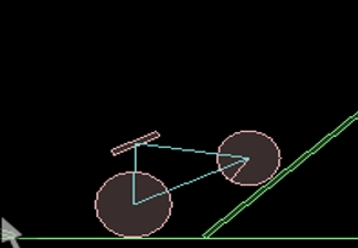
\includegraphics[width=.6\textwidth,center]{./Screenshots/bike.jpg}
  \end{figure}
\end{frame}

\begin{frame}
\frametitle{Divisions}
\framesubtitle{Bike}
  \textbf{Bike} \pause
  \begin{itemize}
    \item Engineering the shock absorbers for the Bike. \pause
    \item Monitoring the interaction of the bike with the terrain in accordance with the physics laws. \pause
    \item Ofcourse, friction providing angular and linear velocity to the Bike. \pause
  \end{itemize}
\texttt{1. } $ \overrightarrow{\tau} = I\overrightarrow{\alpha} = \frac{d \overrightarrow{L}}{dt} $  \pause where \\
  $ \overrightarrow{\tau} $: Torque provided \\
  $ I $: Moment of Inertia of the body \\
  $ \overrightarrow{\alpha} $: Angular acceleration of the body \\
  $ \overrightarrow{L} $: Angular Momentum of the body 
\end{frame}

\begin{frame}
\frametitle{Divisions}
\framesubtitle{Car}
  \textbf{Car}
  \begin{figure}
  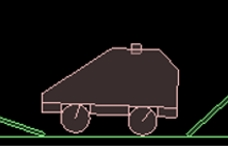
\includegraphics[width=.6\textwidth,center]{./Screenshots/car.jpg}
  \end{figure}
\end{frame}

\begin{frame}
\frametitle{Divisions}
\framesubtitle{Car}
  \textbf{Car} \pause
  \begin{itemize}
    \item Motion of Car can be approximated as the motion of its Centre of Mass. \pause
    \item Car will have a linear velocity assumed to be generated by its engine which is subjected to external forces for acceleration or decceleration. \pause
    \item Car is sufficiently heavy to avoid toppling. \pause  
    \item Pure rolling governed by Friction Laws of the wheels of Car. \pause
  \end{itemize}
 \texttt{2. } $ \overrightarrow{v} = \overrightarrow{u} + \overrightarrow{a}.t $ \pause where \\
  $ \overrightarrow{v} $: Final velocity vector \\
  $ \overrightarrow{u} $: Initial velocity vector \\
  $ \overrightarrow{a} $: CONSTANT Acceleration vector \\
  $ t $: time for which body acts under the effect of the acceleration
\end{frame}

\begin{frame}
\frametitle{Divisions}
\framesubtitle{Tank}
  \textbf{Tank}
  \begin{figure}
  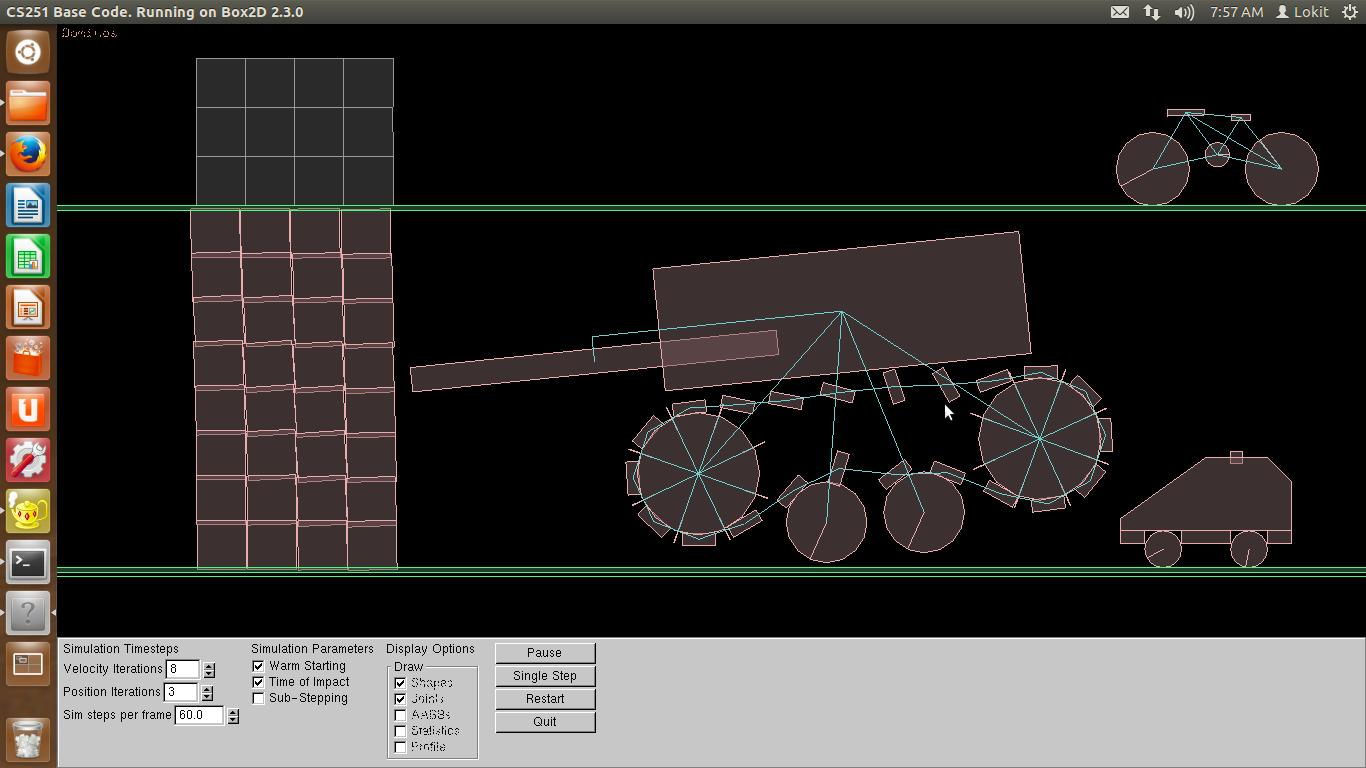
\includegraphics[width=.8\textwidth,center]{./Screenshots/tank.jpg}
  \end{figure}
\end{frame}
 
\begin{frame}
\frametitle{Divisions}
\framesubtitle{Tank}
  \textbf{Tank} \pause
  \begin{itemize}
    \item The vehicular chain of the Tank is modelled as a {\em Conveyor Belt}. \pause
    \item The Impulse on collision with Tank is huge as Tank is sufficiently heavy. \pause
    \item The mechanical structure of Tank is intentionally made strong to exhibit its battlefield endurance. \pause 
    \item If time permits, designing of the Rocket Launching System for the Tank. \pause
  \end{itemize}
 \texttt{3. } $ e = \frac{v_1 - v_2}{u_1 - u_2} $ \pause  where \\
  $ v_1 $: Final velocity of body 1 \\
  $ v_2 $: Final velocity of body 2 \\
  $ u_1 $: Initial velocity of body 1 \\
  $ u_2 $: Initial velocity of body 2 \\
  $ e $: Coefficient of Restitution \\
  \alert{Note:} All velocities along the direction of collision
\end{frame}

\begin{frame}
\frametitle{Divisions}
\framesubtitle{Terrain}
  \textbf{Terrain}
  \begin{figure}
  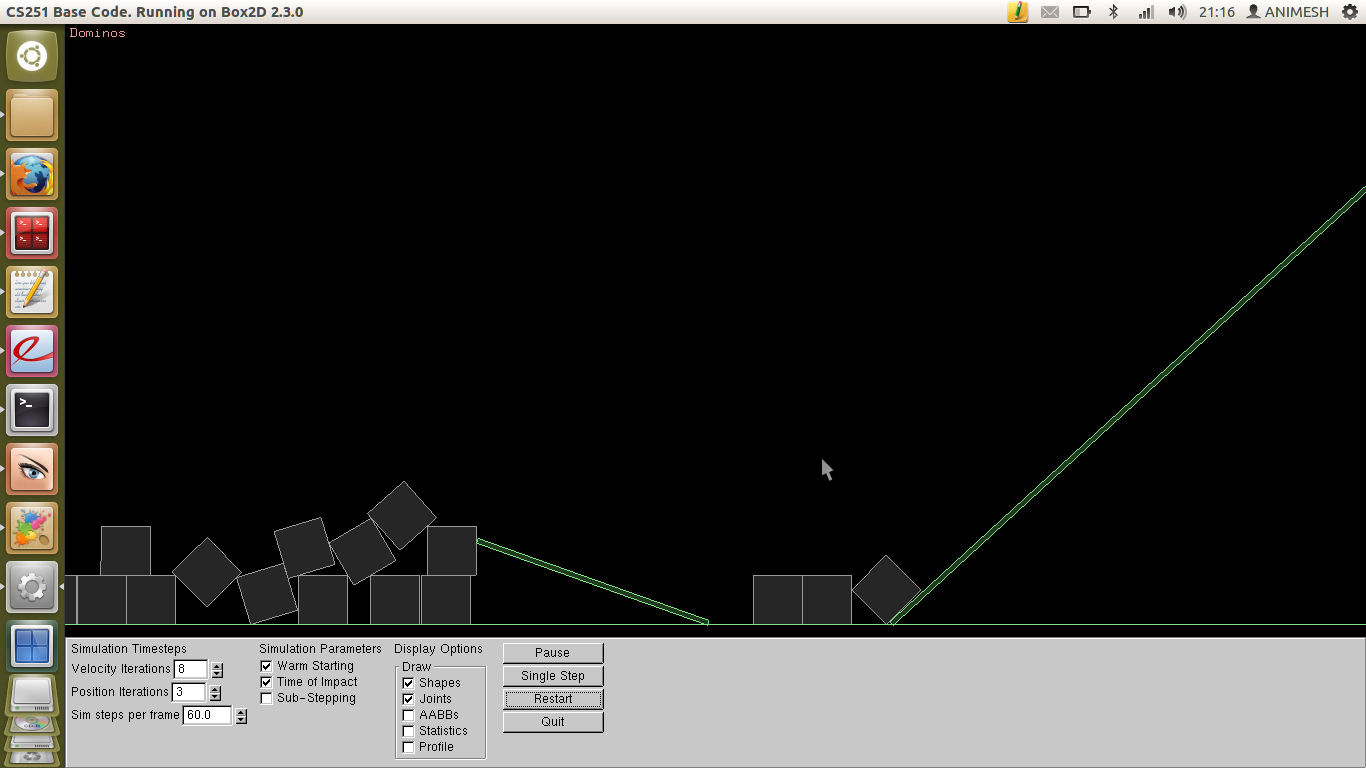
\includegraphics[width=.8\textwidth,center]{./Screenshots/terrain.png}
  \end{figure}
\end{frame}

\begin{frame}
\frametitle{Divisions}
\framesubtitle{Terrain}
  \textbf{Terrain} \pause
  \begin{itemize}
    \item Ramps and pits provided on terrain to alter the velocity of the vehicles. \pause 
    \item Various obstacles on terrain to hinder vehicles. \pause
    \item Macroscopic version of spheres, dominoes to give a feel of \textbf{Rude Goldberg} machine. \pause
  \end{itemize}
 \texttt{4. } $ m_1\overrightarrow{v_1} + m_2\overrightarrow{v_2} = m_1\overrightarrow{u_1} + m_2\overrightarrow{u_2} $ \pause  where \\
  $ \overrightarrow{v_1} $: Final velocity of body 1 \\
  $ \overrightarrow{v_2} $: Final velocity of body 2 \\
  $ \overrightarrow{u_1} $: Initial velocity of body 1 \\
  $ \overrightarrow{u_2} $: Initial velocity of body 2 \\
  $ m_1 $: Mass of body 1 and $ m_2 $: Mass of body 2 \\
  This is the \textbf{Law of Momentum Conservation}.
\end{frame} 

\begin{frame}
\frametitle{The Final Picture}
\begin{itemize}
  \item Helps us in visualising physical laws in a virtual environment. \pause
  \item Introduces an interesting version of a Rube Goldberg Machine. \pause
  \item In the end, the project gives us a brief view of how vehicular models can be tested in virtual environments. \pause 
\end{itemize}
\end{frame}

\begin{frame}
\frametitle{REFERENCES}
\begin{itemize}
  \item BOX 2D TUTORIALS : \cite{link1} 
  \item INSPIRED BY THE BIKE VIDEO : \cite{link2} 
  \item HELPED BY DISCUSSIONS ON THE FORUM : \cite{link3}
\end{itemize}
\end{frame}

\bibliography{reference}{}
\bibliographystyle{plain}

%\input{reference.tex}
\end{document}


